%%%%%%%%%%%%%%%%%%%%%%%%%%%%%%%%%%%%%%%%%%%%%%%%%%%%%%%%%%%%%%%%
%
% Copyright (C) 2013 Roberto Velasco Segura and Pablo L. Rendon.
%
% This file is provided to you under the Creative Commons
% Attribution-Noncommercial-ShareAlike license
%
% http://creativecommons.org/licenses/by-nc-sa/3.0/legalcode
%
% A version of this file has been previously published in
% http://arxiv.org/abs/1311.3004
%
%%%%%%%%%%%%%%%%%%%%%%%%%%%%%%%%%%%%%%%%%%%%%%%%%%%%%%%%%%%%%%%%

%%% \MDbegin*{journalX}
% \documentclass[12pt, titlepage, reqno]{article}
% \usepackage[super]{natbib}
% \usepackage{amssymb}
% \usepackage{amsmath} 
% \usepackage{amsthm}
% \usepackage{bm}
% \usepackage[mathscr]{eucal}
% \usepackage{enumerate}
% \renewcommand{\thefootnote}{\alph{footnote})}    
% \renewcommand{\baselinestretch}{2}
% \renewcommand{\section}[1]{\medskip \addtocounter{section}{1}\raggedright 
%   \textbf{\Roman{section}. \ #1}\medskip \setcounter{subsection}{0}
%   \setlength{\parindent}{5ex}
% }
% \renewcommand{\subsection}[1]{\medskip \addtocounter{subsection}{1}\raggedright
%   \textbf{\Alph{subsection}. \ #1} \medskip \setcounter{subsubsection}{0}\setlength{\parindent}{5ex}
% }
% \renewcommand{\bibsection}{\medskip \raggedright  \textbf{REFERENCES} \medskip}
% \renewcommand{\bibnumfmt}[1]{\textbf{{#1}.}\ \ }
% \pagestyle{myheadings}
% \markboth{\hfill Velasco-Segura and Rend\'{o}n, p.\ }{\hfill Velasco-Segura and Rend\'{o}n, p.\ }
% \setlength{\parindent}{5ex}
% \setlength{\paperwidth}{8.5in}
% \setlength{\textwidth}{6.5in}
% \setlength{\oddsidemargin}{0in}
% \setlength{\evensidemargin}{0in}

% \usepackage{graphicx}
% \usepackage[utf8]{inputenc}
% \usepackage{multirow}
% \usepackage{url} 
%%% \MDend*{journalX}


%%% \MDbegin{twoColumnB}
% \documentclass[letterpaper,twocolumn]{article}
% \usepackage{amssymb}
% \usepackage{amsmath}
% \usepackage[comma]{natbib}
% \setcitestyle{square}
% \usepackage{graphicx}
% \usepackage[utf8]{inputenc}
% \usepackage{setspace}
% \usepackage{multirow}
% \usepackage{url} 
% \textwidth=7.2in
% \oddsidemargin=-0.4in
% \newcommand{\CustomAbstract}[1]{
% \twocolumn[
% \begin{@twocolumnfalse}
%   #1
% \end{@twocolumnfalse}
% ]
% } 
% \let\oldcaption\caption
% \renewcommand{\caption}[1]{\oldcaption{\footnotesize #1}}
% \topmargin = -0.9in
% \textheight = 9.7in
%%% \MDend{twoColumnB}


%%% \MDbegin{phone} 
\documentclass[12pt]{article}
\usepackage[a6paper]{geometry}
\usepackage{amssymb}
\usepackage{amsmath}
\usepackage[comma]{natbib}
\setcitestyle{square}
\usepackage{graphicx}
\usepackage[utf8]{inputenc}
\usepackage{setspace}
\usepackage{multirow}
\usepackage{url} 
\oddsidemargin= -0.97in 
\topmargin=-1.5in
\textheight=5.7in
\textwidth = 4.05in
\let\oldcaption\caption
\renewcommand{\caption}[1]{\oldcaption{\footnotesize #1}}
%%% \MDend{phone} 


%%% \MDbegin{preprint}
% \documentclass[preprint]{jasatex}
% \usepackage{amssymb}
% \usepackage{amsmath}
% \usepackage{graphicx}
% \usepackage[utf8]{inputenc}
% \usepackage{setspace}
% \usepackage{multirow}
% \usepackage{url}
%%% \MDend{preprint}


%%% \MDbegin{twoColumnA}
% \documentclass[nopreprint]{jasatex}
% \usepackage{amssymb}
% \usepackage{amsmath}
% \usepackage{graphicx}
% \usepackage[utf8]{inputenc}
% \usepackage{setspace}
% \usepackage{multirow}
% \usepackage{url}
%%% \MDend{twoColumnA}


%%% \MDbegin{tablet}
% \documentclass[a5paper]{article}
% \usepackage{amssymb}
% \usepackage{amsmath}
% \usepackage[comma]{natbib}
% \setcitestyle{square}
% \usepackage{graphicx}
% \usepackage[utf8]{inputenc}
% \usepackage{setspace}
% \usepackage{multirow}
% \usepackage{url} 
% \oddsidemargin= -0.6in 
% \topmargin=-1.2in
% \textheight=7.1in
% \textwidth = 5in
% \let\oldcaption\caption
% \renewcommand{\caption}[1]{\oldcaption{\footnotesize #1}}
%%% \MDend{tablet}


%%% \MDbegin*{arXiv}
% \documentclass[nopreprint]{jasatex}
% \usepackage{amssymb}
% \usepackage{amsmath}
% \usepackage{graphicx}
% \usepackage[utf8]{inputenc}
% \usepackage{setspace}
% \usepackage{multirow}
% \usepackage{url} 
%%% \MDend*{arXiv}

\pdfoutput=1

\usepackage{my-private}

%%% \MDbegin{phone preprint tablet twoColumnA twoColumnB}
%% \usepackage{bib-at-work}
%%% \MDend{phone preprint tablet twoColumnA twoColumnB}

\begin{document}%%%%%%%%%%%%%%%%%%%%%%%%%%%%%%%%%%%%%%%%%%%%%%%

%%% \MDbegin{journalX}
% \begin{titlepage}
%   \begin{center}

%     \textbf{A finite volume approach for the simulation of nonlinear dissipative acoustic wave propagation} 
%     % running title:
%     % Finite volume nonlinear acoustic propagation

%     \vspace{10ex}

%     {Roberto Velasco-Segura} and
%     {Pablo L. Rend\'{o}n}\footnote{
%       Author to whom correspondence should be addressed. 
%       Electronic mail: pablo.rendon@ccadet.unam.mx
%     } \\

%     Grupo de Ac\'{u}stica y Vibraciones, \\
%     Centro de Ciencias Aplicadas y Desarrollo Tecnol\'{o}gico, \\
%     Universidad Nacional Aut\'{o}noma de M\'{e}xico, \\
%     Ciudad Universitaria–M\'{e}xico, D.F. 04510 M\'{e}xico

%     PACS: {43.25.Cb, 43.58.Ta}
%     \date{\today}
%   \end{center}
% \end{titlepage}
%%% \MDend{journalX}

%%% \MDbegin{twoColumnB phone tablet}
\title{A finite volume approach for the simulation of nonlinear dissipative acoustic wave propagation} 

\author{Roberto Velasco-Segura \\ 
\and Pablo L. Rend\'{o}n}

\date{\today}
\maketitle
%%% \MDend{twoColumnB phone tablet}

%%% \MDbegin{preprint twoColumnA arXiv}
% \title[Finite volume nonlinear acoustic propagation]{A finite volume approach for the simulation of nonlinear dissipative acoustic wave propagation} 
%
% \author{Roberto Velasco-Segura}
% \author{Pablo L. Rend\'{o}n}
% \email[Author to whom correspondence should be addressed. 
% Electronic mail: ]{pablo.rendon@ccadet.unam.mx}
%
% \affiliation{Grupo de Ac\'{u}stica y Vibraciones, Centro de Ciencias Aplicadas y Desarrollo Tecnol\'{o}gico, Universidad Nacional Aut\'{o}noma de M\'{e}xico, Ciudad Universitaria–M\'{e}xico, D.F. 04510 M\'{e}xico}
%
% \pacs{43.25.Cb, 43.58.Ta}
% \date{\today}
%%% \MDend{preprint twoColumnA arXiv}

\begin{abstract}
  A form of the conservation equations for fluid dynamics is presented, deduced using slightly less restrictive hypothesis than those necessary to obtain the well known Westervelt equation. 
  This formulation accounts for full wave diffraction, nonlinearity, and thermoviscous dissipative effects. 
  A 2D finite volume method using the Roe linearization was implemented to obtain numerically the solution of the proposed equations. 
  In order to validate the code, two different tests have been performed: 
  one against a special Taylor shock-like analytic solution, 
  the other against published results on a HIFU system, 
  both with satisfactory results. 
  The code is written for parallel execution on a GPU, thus improving performance by a factor of over 60 when compared to a standard serial execution finite volume code.
\end{abstract}

%%% \MDbegin{preprint twoColumnA arXiv}
% \maketitle
%%% \MDend{preprint twoColumnA arXiv}

%%% \MDbegin{journalX}
% \addtocounter{page}{2}
%%% \MDend{journalX}

\section{Introduction}  
\label{sec:introduction} 

%%% \MDbegin{journalX}
% \setlength{\parindent}{5ex}
%%% \MDend{journalX}

Conservation principles constitute the main starting point for the obtention of the fundamental equations in acoustics. 
A wide variety of acoustic phenomena can be modeled by adding certain hypotheses to these principles in accordance with the characteristics of both the medium involved and the type of solution sought. 
Since these hypotheses generally take the form of restrictions, some models are more restrictive than others, but they usually posses solutions which are more easily found and expressed, {\em e.g.} the linear hypothesis leads to the well known linear wave equation and its general analytic solutions. 
When the linear hypothesis is relaxed, the resulting equations will involve nonlinearity to some degree. 
The better known equations of this type are, listed from less to more restrictive \citep{clason2009boundary, hamilton1998model}:
the Kuznetsov equation \citep{kuznetsov1971equations}, 
the Westervelt equation \citep{westervelt}, 
the KZK equation \citep{kuznetsov1971equations,zabolotskaya1969quasi}, 
and the Burgers equation. 
Of fundamental importance in distinguishing between these equations are the directions of propagation allowed. 
After the Westervelt equation, the hypothesis necessary in order to permit simplification of the model and obtention of the KZK and Burgers equations, is a restriction to propagation at small angles from a certain axis (quasi-planar propagation) in the case of the KZK equation, and strictly along the axis (planar propagation) for the Burgers equation \citep{hamilton1998model}. 
Other nonlinear acoustic models take into account the joint effects of nonlinearity and different properties of the medium, such as 
the presence of bubbles \citep{sutin1998nonlinear}, 
relaxation processes \citep{johnson2003effect}, 
dispersion in shallow water \citep{infeld2000nonlinear}, 
and frequency-dependent absorption in tissues \citep{duck}. 
Furthermore, many of these models have extensions for special cases, {\em e.g.} the Burgers equation can be generalized to describe cylindrical and spherical propagation \citep{crighton1979asymptotic}.

With a few notable exceptions, solutions for all of these nonlinear equations, when known, can only be expressed in non trivial forms, and tools like numeric methods are often required to investigate their nature. 
Numeric methods, and the means required to implement them, have been in continuous development in recent years. 
As a consequence, many publications have been devoted to the description of the more restricted models, like the plane Burgers equation \citep{crighton1979asymptotic}, whose exact solution has known analytical expressions \citep{crighton1979asymptotic, blackstock1966connection, jordan}. 
Nevertheless, even in this case, numeric methods have certainly played an important role \citep{yang1992comparative}. 
Afeter that, the KZK equation became a widely used model for diagnostic and therapeutic medical applications \citep{duck}, and most of the known solutions have been obtained only by numerical means \citep{khokhlova2001numerical}, including some more recent extensions of the model where the restrictions in propagation direction have been partly relaxed \citep{yuldashev2011simulation, dagrau2011acoustic, varray2011fundamental, varslot2005computer}. 
Modern medical applications, such as extracorporeal shock wave therapy \citep{fagnan2008high}, focus control of high intensity focused ultrasound (HIFU) in heterogeneous media \citep{okita2011development}, and ultrasound imaging \citep{huijssen2010iterative}, are now demanding more sophisticated solutions to describe systems where the geometric complexity of the nonlinear acoustic field is important. 
Thus, in recent years, a number of schemes have been produced concerned with implementing methods which are not restricted in terms of the propagation direction \citep{christopher1991new, albin, demi2011contrast, okita2011development, huijssen2010iterative, karamalis, hallaj1999fdtd, pinton2009heterogeneous}, as required in order to solve the Westervelt and Kuznetsov equations. 
These are sometimes referred to as full wave methods \citep{hallaj1999fdtd}. 
To the best of our knowledge, no general analytic solutions are known for the full wave case either for the Kuznetsov or the Westervelt equations. 
In the present work we aim to give a full wave numerical solution to a set of conservation laws, obtained using slightly less restrictive hypotheses than those necessary to arrive at the Westervelt equation. 
As a first step, our scheme has been implemented only for a homogeneous medium.

A great number of numeric methods have been used to solve the nonlinear acoustic field, some of them operating over time domain \citep{karamalis, hallaj1999fdtd, okita2011development, pinton2009heterogeneous}, while others involve calculations over the frequency domain \citep{christopher1991new, albin, varray, varray2011fundamental, demi2011contrast}.  
The numeric method developed in the present work is a finite volume method, a time domain method. 
These methods are based on conservation laws, giving them from the start an intrinsic relation to the equations that conform the basis of all acoustic wave models. 
Finite volume methods have been successfully applied in systems exhibiting nonlinear propagation effects, such as 
shallow water waves \citep{rjl-george:catalina04}, 
vehicle traffic flow \citep{yi2003stability}, 
and acoustic propagation \citep{christov}, among others. 
In the present work, the CLAWPACK \citep{clawpack} code, which serves as a standard for finite volume schemes, has been used solely as a reference for execution time. We have written a C++/CUDA code, described in the following sections, to execute the finite volume method in a GPU graphic card, which notably improves overall performance compared to serial schemes such as the one mentioned above. 
Whereas in the recent literature it is a common practice to use parallelized code for this kind of simulations, this code is mainly run through clusters \citep{albin,  huijssen2010iterative, yuldashev2011simulation, okita2011development, varslot2006forward, pinton2009heterogeneous}, and GPU execution is just starting to be used \citep{varray, cudaclaw, karamalis}. 
The paper is organized as follows: 
the relevant equations for this study are described in Section~\ref{sec:equations}; the numeric procedure is described in Section~\ref{sec:numerical}; 
validation tests for the numeric method, and details of their implementation, are given in Section~\ref{sec:results}, 
and discussion and conclusions are presented in Section~\ref{sec:disc-concl}. 
Finally, the details for obtaining the set of equations we propose are included in Appendix~\ref{sec:appendix}.

\section{Equations}
\label{sec:equations}

The Westervelt equation is a classical model for nonlinear acoustic propagation, and in standard form is given as \citep{hamilton1998model}
\begin{align}
  \label{eq:Westervelt}
  \nabla^2 p' 
  - \frac{1}{c_0^2}\Dp{^2 p'}{t^2}
  + \frac{\delta}{c_0^4} \Dp{^3 p'}{t^3} 
  =
  \frac{-\beta}{\rho_0 c_0^4} \Dp{^2 (p')^2}{t^2}
  \p{,}
\end{align}
where $p'$ is the acoustic perturbation pressure, $\nabla^2$ is the Laplacian for spatial variables, $t$ is time, $c_0$ is speed of sound for small signals, $\beta$ is the coefficient of nonlinearity \citep{beyer1998parameter}, $\delta$ is sound diffusivity \citep{lighthill} (see Appendix~\ref{sec:appendix}).
It was originally obtained in 1963 by P. J. Westervelt \citep{westervelt} and describes an acoustic propagation taking into account the competing effects of nonlinearity and attenuation, the relative magnitude of which are given by the values of the coefficients $\beta$ and $\delta$ respectively.

As described by Hamilton and Morfey \citep{hamilton1998model}, the Westervelt equation can be obtained from the conservation laws for a viscid compressible fluid, assuming the following set of hypotheses:
(i) the flow is irrotational,
(ii) the equilibrium state of the fluid has null flow, 
(iii) the perturbation expansion can be truncated at orders $\epsilon^2$ and $s'$ (where $\epsilon$ is the Mach number $\epsilon = u/c_0$, with $\mathbf{u}$ a typical particle velocity, and $s'$ is the specific entropy deviation over the equilibrium state),
(iv) the ratios of the perturbation values over the equilibrium values are of order $\epsilon$ for $\rho$ (density), $p$ (pressure), and $T$ (temperature),
(v) first-order relations can be used in the second-order equations; 
and finally, (vi) the Lagrangian density can be neglected. 
We have used the same hypotheses, except for the last one, over the same initial set of conservation laws, to obtain a different form of these conservation laws, as follows:
\begin{subequations}
\label{eq:OurSystem}
\begin{align} 
  \label{eq:mod-prop-fin-mas}
  \frac{\partial \rho}{\partial t} + \nabla \cdot
  \left(\rho \mathbf{u}\right)& = 0 
  \p{,} \\ 
  \label{eq:mod-prop-fin-mom}
  \Dp{\rho \mathbf{u}}{t} +
  \nabla\cdot\left(
    \rho_0 \mathbf{u}\otimes\mathbf{u} + \mathbf{I}\tilde{p}
  \right)
  &= 
  \rho_0 \delta \nabla^2 \mathbf{u}
  \p{,} 
\end{align}
\end{subequations}
where
\begin{align*}
  \tilde{p} = 
  c_0^2 \rho + \frac{c_0^2}{\rho_0} (\beta-1)(\rho-\rho_0)^2 
  \p{,}
\end{align*}
is the associated equation of state, $\otimes$ denotes outer product, and $\mathbf{I}$ is an identity matrix.

Equations of this kind are sometimes called {\em balance laws} because of the presence of the source term \citep{leveque-book-fv}, p. 375, identified above as the right hand side of equation \eqref{eq:mod-prop-fin-mom}. 
A detailed description of the procedure to obtain \eqref{eq:OurSystem} can be found in Appendix~\ref{sec:appendix}. 
The advantage afforded by this balance law system of equations is that permits the implementation of a numerical finite volume method, described in Section~\ref{sec:numerical}, to obtain numerical solutions.
Additionally, the fact that expressions \eqref{eq:OurSystem} were obtained under slightly less restrictive hypotheses than the Westervelt equation, makes them slightly more general and could thus be expected to describe a wider variety of acoustic nonlinear dissipative phenomena.

\section{Numeric method}
\label{sec:numerical}

For the rest of this paper only two spatial dimensions are considered.  The theory presented in Section~\ref{sec:equations} and Appendix~\ref{sec:appendix} is valid for three spatial dimensions, but we have chosen to restrict our implementation, for the moment, to two dimensions, mainly to keep down computational costs.

Using a variable renormalization
\begin{align}
  \label{eq:renorm}
  \frac{t c_0}{L}  \mapsto t
  \p{,} \qquad
   \frac{x_j}{L} \mapsto  x_j
  \p{,} \quad \text{with} \quad
  j = 1,2
\end{align}
where $L$ a is typical length in the system, the equations \eqref{eq:OurSystem} can be rewritten in non-dimensional differential conservation law form \citep{sharma2010quasilinear}, as follows:
\begin{align}
  \label{eq:OurSysAdim}
  \Dp{q}{t} + \Dp{f_1}{x_1} + \Dp{f_2}{x_2} = \psi \p{,}
\end{align}
where $q$ is the vector of conserved quantities, $f_j$ is the vector containing their fluxes, and $\psi$ is a source term. These vectors are written in the following form:
\begin{align*}
  q 
  &=
  \left(
    \begin{array}{c}
      q^1 \\
      q^2 \\
      q^3
    \end{array}
  \right)
  =
  \frac{\rho}{\rho_0}
  \left(
    \begin{array}{c}
      1 \\
      u^1/c_0 \\
      u^2/c_0
    \end{array}
  \right) \p{,}
 \\
  f_j
  &= \frac{q^{j+1}}{(q^1)^2}
  \left(
    \begin{array}{c}
      (q^1)^2 \\
      q^2 \\
      q^3
    \end{array}
  \right)
  + \phi 
  \left(
    \begin{array}{c}
      0 \\
      \delta_{1j} \\
      \delta_{2j}
    \end{array}
  \right) \p{,} \\
  \phi &= q^1 + (\beta-1)(q^1-1)^2 \p{,} \\
  \psi
  &=
  \tilde{\delta}
  \left(
    \begin{array}{c}
      0 \\
      \nabla^2 q^2/q^1 \\
      \nabla^2 q^3/q^1
    \end{array}
  \right) \p{,}
\end{align*}
where $\delta_{ij}$ is a Kronecker delta.

The coefficient 
\begin{align}
  \label{eq:phi-tdelta}
  \tilde{\delta} = \frac{\delta}{c_0 L}
\end{align}
is a dimensionless form of the sound diffusivity $\delta$ as given by Lighthill \citep{lighthill},
and the parameter $\beta$ is the coefficient of nonlinearity \citep{beyer1998parameter}.

In order to implement a fractional step method, which is convenient because it allows us to deal with simpler equations, we use the following decomposition
\begin{align}
  \label{eq:fs:cl1}
  \Dp{q}{t} + \D{f_1}{q}\Dp{q}{x_1} &= 0 \p{,}\\
  \label{eq:fs:cl2}
  \Dp{q}{t} + \D{f_2}{q}\Dp{q}{x_2} &= 0 \p{,}\\
  \label{eq:fs:source}
  \Dp{q}{t} &= \psi \p{,}
\end{align}
where $\D{f_j}{q}$ is a $3\times 3$ Jacobian matrix. 
The fractional step method in this case consists in applying consecutive numerical schemes for equations \eqref{eq:fs:cl1}, \eqref{eq:fs:cl2}, and \eqref{eq:fs:source}.
That is, for every time step, the initial state of the mesh is used in a numerical scheme for the first equation, then the result is used as input for a numerical scheme of the second equation, and so on.
Since \eqref{eq:fs:cl1} and \eqref{eq:fs:cl2} are essentially the same equation, switching positions $2$ and $3$ in every vector, they can be solved numerically with the same scheme. 
For this reason, we have dropped the $j$ subscript in the following sections. To obtain a numerical solution for expression \eqref{eq:fs:source}, a standard central finite difference second-order method was used.

\subsection{Finite volume method}
\label{sec:finite-volume-method}

A numerical solution to equation \eqref{eq:fs:cl1} is sought using a finite volume high-resolution method \citep{leveque-book-fv}, p. 121, of the form
\begin{align}
  \nonumber
  Q_i^{n+1} &= Q_i^n
  -\frac{\Delta t}{\Delta x}
  \left(
    \mathcal{A}^-\Delta Q_{i+1/2}
    + \mathcal{A}^+\Delta Q_{i-1/2}
  \right) \\
  \label{eq:fv-hr}
  & \quad
  -\frac{\Delta t}{\Delta x}
  \left(
    \tilde{F}_{i+1/2}
    -\tilde{F}_{i-1/2}
  \right)
  \p{,}
\end{align}
where, as usual in finite volume methods,
\begin{align*}
  Q^n_i \approx \frac{1}{\Delta x} \int_{x_{i-1/2}}^{x_{i+1/2}} 
  q(x,t_n) \ dx
  \p{.}
\end{align*}
Expression \eqref{eq:fv-hr}, is in principle, a numeric method formulated for a linear system of conservation laws. The procedure needed to use it with a nonlinear system is briefly described below, and further details can be found in LeVeque's textbook \citep{leveque-book-fv}, Chap. 15. 
Expression \eqref{eq:fv-hr} approximates the new values of $q$ in the cell $i$, that is $Q^{n+1}_i$, as a function of the old value $Q^n_i$ and the fluxes from neighboring cells. 
These fluxes are described by the matrix $\D{f(q)}{q}$, which is dependent on $q$ because of the nonlinear character of equation \eqref{eq:OurSysAdim}, and is thus dependent on position.
This matrix is evaluated at $i-1/2$ to determine the flux between cell $i$ and cell $i-1$, and at $i+1/2$ to determine the flux between cell $i+1$ and cell $i$. 
We have implemented a Roe linearization \citep{roe, leveque-book-fv} scheme to approximate this matrix $\D{f(q)}{q}$ at these positions. 
Once we have these approximations, say for $i_{i-1/2}$, their eigenvalues $s_{i-1/2}^p$ and eigenvectors $r_{i-1/2}^p$ can be obtained. Further details are presented in Section~\ref{sec:roe}. 

The second term in expression \eqref{eq:fv-hr} is constructed with terms sometimes called {\em fluctuations} \citep{leveque-book-fv}, p. 80,
\begin{align}
  \label{eq:fluc:m}
  \mathcal{A}^-\Delta Q_{i+1/2} 
  &= \sum_{p=1}^3(s_{i+1/2}^p)^- \mathcal{W}_{i+1/2}^p 
  \p{,}\\
  \label{eq:fluc:p}
  \mathcal{A}^+\Delta Q_{i-1/2} 
  &= \sum_{p=1}^3(s_{i-1/2}^p)^+ \mathcal{W}_{i-1/2}^p
  \p{,}
\end{align}
where 
\begin{align*}
  \mathcal{W}^p_{i-1/2} = \alpha^p_{i-1/2} r^p_{i-1/2}
\end{align*}
and $\alpha^p_{i-1/2}$ just represent a normalization of the eigenvectors $r^p_{i-1/2}$ in order to satisfy
\begin{align*}
  Q_i - Q_{i-1} = \sum_{p=1}^3 \alpha_{i-1/2}^p r^p_{i-1/2}
  \p{.}
\end{align*}
The definitions in equations \eqref{eq:fluc:m} and \eqref{eq:fluc:p} correspond to a Godunov first-order method. What this means is that if the third term of equation \eqref{eq:fv-hr} were absent, and as it is shown below this could eventually happen, then equation \eqref{eq:fv-hr}, because of its second RHS term, would have the form of a Godunov method.

The third term in the RHS of expression \eqref{eq:fv-hr} is a flux limiter \citep{leveque-book-fv}, Chap. 6, of the form
\begin{align}
  \label{eq:limiter}
  \tilde{F}_{i-1/2}
  =
  \frac{1}{2}
  \sum_{p=1}^3
  \left|s_{i-1/2}^p\right|
  \left(
    1-
    \frac{\Delta t}{\Delta x}
    \left|s_{i-1/2}^p\right|
  \right)
  \Wtilde^p_{i-1/2}
  \p{,}
\end{align}
where
\begin{align*}
  \Wtilde^p_{i-1/2} 
  &= \tilde{\alpha}^p_{i-1/2}r^p_{i-1/2} 
  \p{,}
  \\
  \tilde{\alpha}_{i-1/2}^p 
  &= \alpha_{i-1/2}^p \theta_{i-1/2}^p 
  \p{,}
  \\
  \theta_{i-1/2}^p
  &=
  \frac{\mathcal{W}_{I-1/2}^p\cdot\mathcal{W}_{i-1/2}^p}
  {\mathcal{W}_{i-1/2}^p\cdot\mathcal{W}_{i-1/2}^p}
  \p{,}
  \\
  I &=
  \begin{cases}
    i-1 & \text{if } s_{i-1/2}^p > 0  \p{,}\\
    i+1 & \text{if } s_{i-1/2}^p < 0  \p{.}
  \end{cases}
\end{align*}
The idea here is to have a coefficient $\theta_{i-1/2}^p$ that becomes  $1$ when the solution is smooth. When this happens, expression \eqref{eq:fv-hr} is precisely a second-order Lax-Wendroff method, but when the solution has an abrupt change this coefficient becomes zero and we are left with a first-order Godunov method. Most of the time this coefficient is neither $0$ or $1$ -- it approaches one or the other depending on the smoothness of the solution.

When substituting expressions \eqref{eq:fluc:m}, \eqref{eq:fluc:p}, and \eqref{eq:limiter} into equation \eqref{eq:fv-hr}, it is noticeable  that equation \eqref{eq:fv-hr} is a sum over families of waves indexed with $p$. 
This decomposition is just an eigenvector representation of the system.
The coefficient $\theta_{i-1/2}^p$ is related to this representation: it is a normalized projection of $\mathcal{W}_{I-1/2}^p$ over $\mathcal{W}_{i-1/2}^p$. If both are close to each other then $\theta_{i-1/2}^p \approx 1$, as they will have almost the same size and direction, and this would be the case only if the solution for the $p$-th wave family is smooth.

\subsection{Roe linearization}
\label{sec:roe}

As we have previously said, we need a matrix $\hat{A}_{i-1/2}$ which approximates $\D{f}{q}$ at the middle point between $i$ and $i-1$, for any given $i$. 
Since $f$ is a nonlinear function of $q$, it is expected that $\hat{A}_{i-1/2}$ will be a function of $Q_i$ and $Q_{i-1}$.
For the purpose of linearization this matrix is considered constant in a finite volume method constructed for the linear case, as in expression \eqref{eq:fv-hr}.

Two properties are expected of such approximations \citep{leveque-book-fv}, p. 316:
\begin{itemize}
\item consistency, {\em i.e.} convergence to $\D{f}{q}$ when $Q_i\rightarrow{}Q_{i-1}$, and
\item diagonalizability by means of real eigenvalues.
\end{itemize}
The Roe linearization is a technique designed to find a matrix which, apart from the previous properties, satisfies
\begin{align}
  \label{eq:RoeCond}
  f(Q_i) -f(Q_{i-1}) = \hat{A}_{i-1/2} (Q_i  - Q_{i-1})
  \p{,}
\end{align}
which is a useful property because it ensures the method will be conservative. Furthermore, for the shock wave cases, where there is a region with a strong change for a single $p$ wave family, {\em i.e.} much bigger than the changes in other wave families, expression \eqref{eq:RoeCond} implies this $p$-wave is (in the limit) an eigenvector of $\hat{A}_{i-1/2}$, which is the case except for the small regions when two shocks collide \citep{leveque-book-fv}, p. 317.

Now, using a variable change $z=z(q)$,
\begin{align*}
  \left(
  \begin{array}{c}
    z^1 \\
    z^2 \\
    z^3
  \end{array}
  \right)
  =
  \left(
    \begin{array}{c}
      q^1 \\
      q^2 / q^1 \\
      q^3 / q^1
    \end{array}
  \right)
\end{align*}
to define a path 
\begin{align*}
  \hat{z}(\xi) = Z_{i-1} + (Z_i - Z_{i-1}) \xi \p{,}
  \qquad
  \text{where}
  \qquad
  Z_i=z(Q_i) \p{,}
\end{align*}
and performing the integrals
\begin{align*}
  \int_0^1 \frac{f(q(\hat{z}(\xi)))}{d\xi} \ d\xi
  \p{,} \quad
  \int_0^1 \frac{q(\hat{z}(\xi))}{d\xi} \ d\xi
  \p{,}
\end{align*}
the desired matrix, satisfying all of the properties mentioned above, is found: %
{\renewcommand{\arraystretch}{2.5}
\begin{align*}
  \hat{A}_{i-1/2}
  =
  \left(
    \begin{array}{ccc}
      0 & 1 & 0 \\
      -\dfrac{(\Z2)^2}{\Z1} + \Phi
      & 2\dfrac{\Z2}{\Z1} & 0  \\
      -2\dfrac{\Z2\Z3}{\Z1} & \dfrac{\Z3}{\Z1}
      & \dfrac{\Z2}{\Z1}
    \end{array}
  \right)
\end{align*}}
where
\begin{align*}
  \Z{p} = \frac{1}{2}\left(Z^p_{i} + Z^p_{i-1}\right) 
  \quad \text{and} \quad
  \Phi = 1 + 2(\beta-1)(\Z1-1) \p{.}
\end{align*}
The eigenvalues of this matrix are
\begin{align}
  \label{eq:lambda1}
  s_{i-1/2}^1 &= \frac{\Z2}{\Z1}
  + \sqrt{\frac{(\Z2)^2}{(\Z1)^2}
    - 2 \frac{(\Z2)^2}{\Z1} 
    + \Phi
  } \p{,}\\   
  \label{eq:lambda2}
  s_{i-1/2}^2 &= \frac{\Z2}{\Z1}
  - \sqrt{\frac{(\Z2)^2}{(\Z1)^2}
    - 2 \frac{(\Z2)^2}{\Z1} 
    + \Phi
  } \p{,}\\   
  s_{i-1/2}^3 &= \frac{\Z2}{\Z1}
\end{align}
and the respective eigenvectors are not difficult to obtain.  

A limitation of this method is evidenced by analysis of expressions \eqref{eq:lambda1} and \eqref{eq:lambda2}: 
if the perturbations are large enough the eigenvalues become complex, and can no longer be used in the way we have described. 
In practice, we simply stop the simulation whenever this happens. 
We remark that this limitation is not inherent to the linearization, as the eigenvalues of $\D{f}{q}$ present the same problem. 
It may be that this is simply a manifestation of the validity of the perturbation techniques used to obtain equations \eqref{eq:OurSystem}.

\section{Implementation and validation}
\label{sec:results}

The mesh used in all the simulations was Cartesian with $\Delta x_1 = \Delta x_2 = \Delta x$; 
in what follows, only $\Delta x$ is used. 
The value of $\Delta t$ was controlled by the CFL value
\begin{align*}
  \nu = \frac{\Delta t}{\Delta x} \max\{s_{i-1/2}^p\} 
\end{align*}
where the maximum is taken over the entire mesh, in both directions, and over the three possible values of $p$. 
In every time step the value of $\Delta t$ was adjusted, using the $\nu$ calculated in the previous step, to maintain $\nu$ around some {\em wished} value $\nu_W$ and so that its value is always less than 1; see \citep{leveque-book-fv}, p. 96, 312.

Since all the simulations presented in this work use only wave packets, then it is possible to save computational resources by using a mobile domain. 
Following Albin {\em et al.} \citep{albin}, two stages of the simulation were implemented:
in the first stage, from $t=t_0<0$ to $t=t_1>0$, the domain stays still and the boundary condition introduces the propagating wave until it reaches the center of the domain at $t=t_1$; 
in the second stage the domain moves with the propagation wave. 
Additionally, the time scale was adjusted to have $t=0$ when the center of the packet was precisely on the left border, and the value of $t_0$ was chosen for the packet to be numerically zero at  machine precision. 
Making use of this technique the simulations were performed in domains as long as 100 wavelengths.

To validate the code, two sets of tests were performed. 
Firstly, in Section~\ref{sec:agains-analyt-solut}, against a Taylor shock solution \citep{jordan}, which is an analytic plane wave solution. 
This  constitutes a test for nonlinearity and diffusivity, but not for full wave diffraction, because of its plane nature. 
As we have previously said, no analytic solutions showing full wave diffraction are known, to our knowledge. 
Thus, the second set of tests were performed against another numeric solution for a HIFU (high intensity focused ultrasound) system, obtained by a different method by Albin {\em et al.} \citep{albin}, in this case a pseudospectral Fourier continuation method.
The results of this comparison are presented in Section~\ref{sec:agains-anoth-numer}.

The present code is written in C++/CUDA v5.0, and it was executed on a Tesla C2075 GPU graphic card (448 cores and 6GB on RAM), installed on a standard PC i3-550 with 16GB on RAM, running Debian/Sid. 
The finite volume code used for performance comparison, described in Section~\ref{sec:performance}, was executed on the same computer.
All the simulations presented here were performed with double precision.  

\subsection{Validation against a plane wave analytic solution}
\label{sec:agains-analyt-solut}

\begin{figure}[htb] 
\centering 
\framebox{
  \resizebox{3.3in}{!}{
    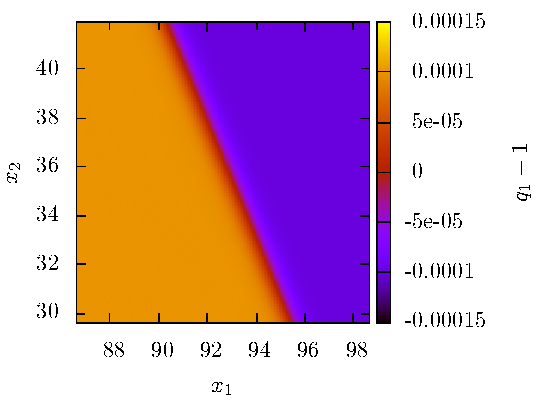
\includegraphics{1.pdf}
  }
} 
\caption{Taylor shock, upper view, numeric solution for $\theta_T = \pi/8$, $\eta=82$ and $t=100$ (color online).}
\label{fig:taylor-upper}
\end{figure}

\begin{figure}[htb] 
\centering 
\framebox{
  \resizebox{3.3in}{!}{
    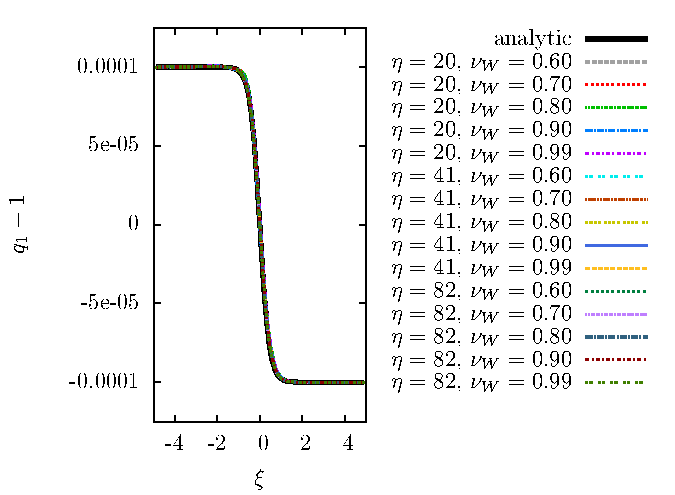
\includegraphics{2.pdf}
  }
} 
\caption{Taylor shock, transverse cut for $\theta_T=\pi/8$ at
  $t=100$, numeric and analytic solutions for different values
  of $\eta$ and $\nu_W$ (color online).}
\label{fig:taylor-transverse}
\end{figure}

\begin{figure}[htb] 
\centering 
\framebox{
  \resizebox{3.3in}{!}{
    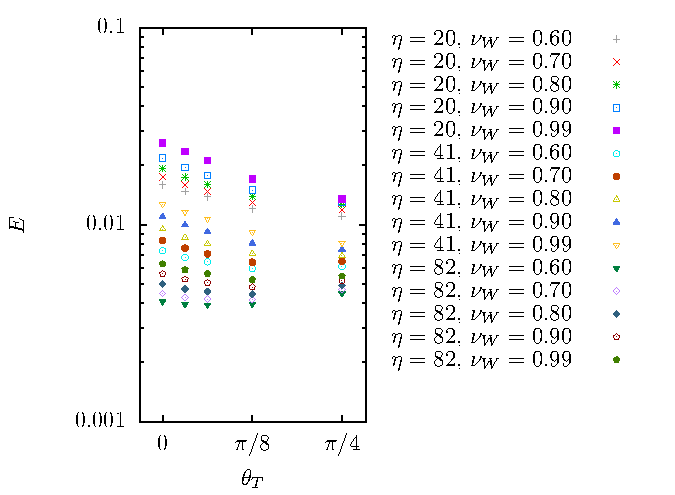
\includegraphics{3.pdf}
  }
} 
\caption{Taylor shock, error $E$ for different values of
  $\theta_T$, $\eta$ and $\nu_W$ (color online).}
\label{fig:taylor-error}
\end{figure}


It is straightforward to verify that
\begin{align*}
  p' &= \frac{-\tilde{\delta}}{\beta} \tanh(x-t) \p{,}
\end{align*}
the sometimes called Taylor shock \citep{jordan}, is a traveling wave solution of the dimensionless version of the Westervelt equation \eqref{eq:Westervelt},
\begin{align*}
  \nabla^2 p' 
  - \Dp{^2 p'}{t^2}
  + \tilde{\delta} \Dp{^3 p'}{t^3} 
  =
  -\beta \Dp{^2 (p')^2}{t^2}
  \p{,}
  \quad \text{for} \quad \frac{p'}{c_0^2\rho_0} \mapsto p'
\end{align*}
where \eqref{eq:renorm} and \eqref{eq:phi-tdelta} were used.  
It is then reasonable to expect that a similar expression could be a solution to equations \eqref{eq:OurSysAdim}. After some algebra it can be shown that
\begin{subequations}
  \label{eq:OurTaylorS}
  \begin{align}
    q^1 &= 1-\frac{\tilde{\delta}}{\beta}\tanh(x-t) \p{,} \\
    q^2 &= q^1 - 1 \p{,}\\
    q^3 &= 0 \p{,}
  \end{align}
\end{subequations}
represent indeed a traveling wave solution to expression \eqref{eq:OurSysAdim} in the following sense: 
equations \eqref{eq:OurSystem}, and consequently \eqref{eq:OurSysAdim}, were obtained neglecting $O(\epsilon^3)$ terms (see Appendix~\ref{sec:appendix}).
When expressions \eqref{eq:OurTaylorS} are substituted in \eqref{eq:OurSysAdim}, only $O(\epsilon^3)$ terms remain, and these terms can thus be neglected at the same approximation order.

For the simulations in this section, all the boundary conditions (left, right, top, and bottom) were taken to be of the form of the analytic solution \eqref{eq:OurTaylorS}, for both stages. As can be seen from equation \eqref{eq:OurTaylorS}, in this case the independent values of $\beta$ and $\tilde{\delta}$ are not important -- only their ratio is. For all following simulations, we have chosen $\tilde{\delta}/\beta = 10^{-4}$.

It is a well-known fact that there are issues concerning the propagation direction in Cartesian meshes \citep{huijssen2010iterative,pinton2009heterogeneous}, because at cell scale the simulation fluxes are horizontal or vertical, but never diagonal. 
In order to appreciate whether these issues pose a problem for our code or not, we tested propagation at several propagation angles $\theta_T$, measured from the $x_1$-axis: 
$0$, $\pi/32$, $\pi/16$, $\pi/8$, $\pi/4$. 
These angles are thought to be representative of most of the relevant possibilities because of the symmetries of the numeric method: 
propagation at $\theta_T=0$ is aligned with the mesh in the same way as propagations at $\theta_T=\pi/2,\pi,3\pi/2$ are. 
Also, since spatial variables can be interchanged, a variety of other angles are equivalent: for example, propagations with $\theta_T$ values $\pi/16$ and $\pi/2 - \pi/16$ would yield the same results.  
Equations \eqref{eq:OurTaylorS}, as they are, correspond to $\theta_T=0$; to use them with a different value of $\theta_T$, we have applied a standard rotation change of variables.

Other important parameters with respect to quality of results are $\nu_W$ and $(\Delta x)^{-1}$. With regard to the former, we recall that the value $\nu_W$ only approximates the real CFL value $\nu$. 
In order to calculate this difference, its standard deviation was measured, with the result that it never exceeded the value $10^{-8}$.
Regarding the latter, for which we use letter $\eta = (\Delta x)^{-1}$, the value of $L$, in equation \eqref{eq:renorm}, was chosen as the distance between points of the wave such that the amplitude at these points is $10\%$ and $90\%$ of the maximum amplitude. 
In dimensionless variables the distance then equals $1$, and in this case $\eta$ then represents the number of cells across the shock wave.

Figure~\ref{fig:taylor-upper} shows how a typical simulation looks like, in this case for $\theta_T = \pi/8$, $\eta=82$, and $t=100$, that is, after the wave has traveled a distance $100$ times larger than its width. 
In figure~\ref{fig:taylor-transverse} transverse cuts are shown, all of them also for $\theta_T=\pi/8$ and $t=100$, over a $\xi$-axis normal to the propagation, but for different values of $\nu_W$ and $\eta$. 
A very good agreement is observed, in figure \ref{fig:taylor-transverse}, for $\theta_T=\pi/8$, and similar agreement is observed for the rest of the tested $\theta_T$ values.

Figure \ref{fig:taylor-error} depicts an error analysis for the
same cases. The error is calculated as \citep{jing2011evaluation}
\begin{align}
  \label{eq:error}
  E = \frac{\| \text{numeric solution}- \text{reference}\|}
    {\|\text{reference}\|} \p{,}
\end{align}
where reference is the analytic solution, and $\|\cdot\|$ stands for the L2 norm, in this case integrated over a 10-unit length centered along a straight line normal to the propagation, as shown in figure \ref{fig:taylor-transverse}, for $t=100$. 
It can be observed that the error in all cases is below $3\%$, and for our finest mesh, with $\eta=82$, the error is below $1\%$, so that we may consider our numeric solution to be in very good agreement with the analytic solution.
Its behavior as a function of $\eta$ and $\nu_W$ is monotonically decreasing as the mesh is refined, that is, when $\nu_W \rightarrow 0$ and $\eta \rightarrow \infty$.

In spite of this, it is not always a good idea to use a low $\nu_W$ value, as in some cases larger values would not much increase the error and would certainly make the simulation faster.  Tests for $\nu_W>1$ were attempted, but they yielded only unstable results.

In Figure \ref{fig:taylor-error} we appreciate that $E$ as a function of $\theta_T$ is not monotonic, and depends, rather, on mesh refinement, but we can also see that the impact of $\theta_T$ on the error is smaller as the mesh is refined, and even in the worst of the presented cases the error is still less than $3\%$.

\subsection{Validation against another set of full wave numeric results}
\label{sec:agains-anoth-numer}

\begin{figure*}[htb] 
\centering 
\framebox{
  \resizebox{\textwidth}{!}{
    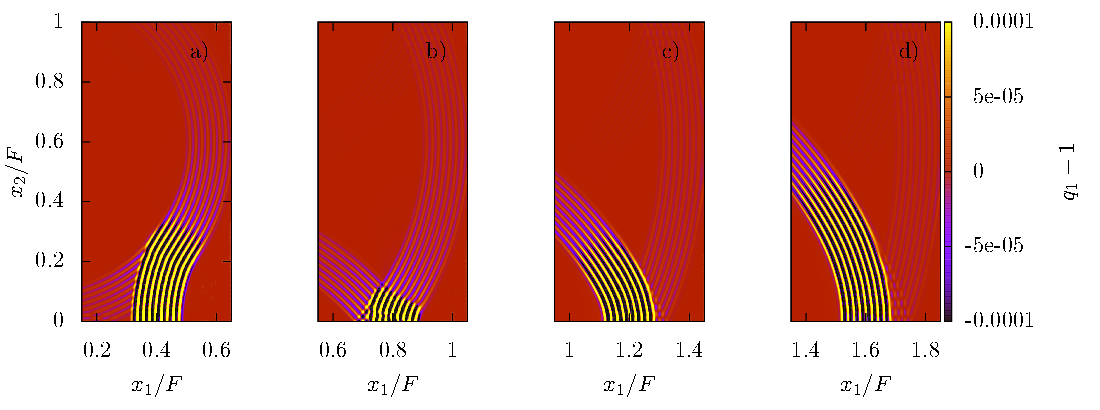
\includegraphics{4.pdf}
  }
} 
\caption{Focused wave, upper view of numeric results for $q^1-1$,  with $a=30$, and a) $t=20$, b) $t=40$, c) $t=60$, d)  $t=80$. Scale for $q_1-1$ is compressed to make edge waves more visible (color online).}
\label{fig:hifu-upper}
\end{figure*}

%%%%%%%%%%%
\begin{figure}[htb] 
\centering 
\framebox{
  \resizebox{3.3in}{!}{
    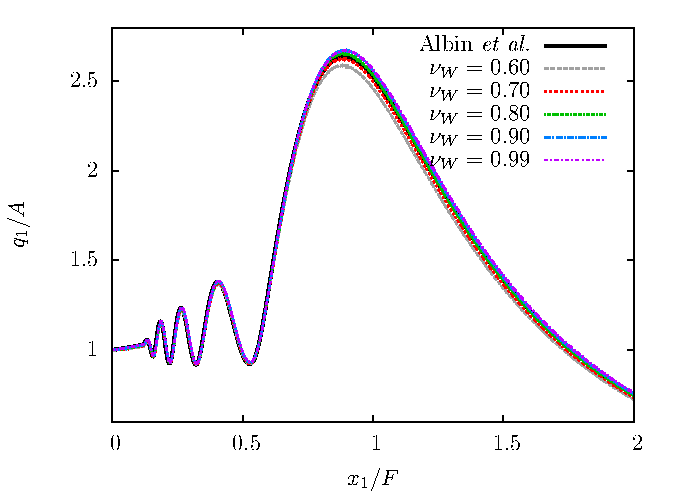
\includegraphics{5.pdf}
  } 
} 
\caption{Focused wave, on axis pressure maximum for $a=10$, $\eta=82$, and different values of $\nu_W$. Reference values taken from Albin {\em et al.} \citep{albin} (color online).}
\label{fig:hifu-u1max-a10}
\end{figure}
%%%%%%%%%%%
\begin{figure}[htb] 
\centering 
\framebox{
  \resizebox{3.3in}{!}{
    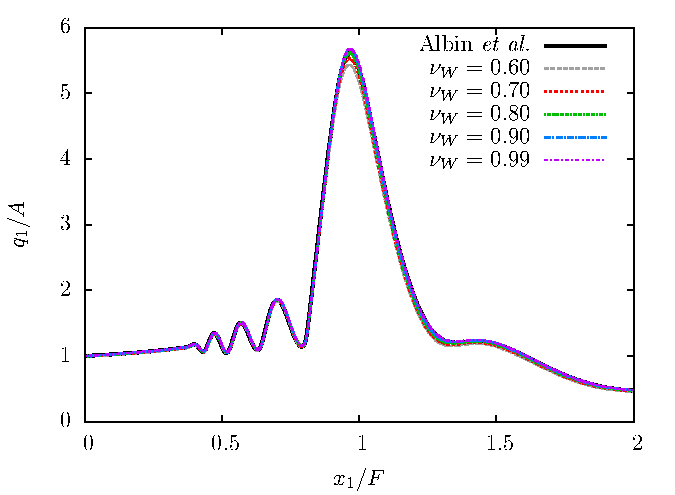
\includegraphics{6.pdf}
  }
} 
\caption{Focused wave, on axis pressure maximum for $a=20$, $\eta=82$, and different values of $\nu_W$. Reference values taken from Albin {\em et al.} \citep{albin} (color online).}
\label{fig:hifu-u1max-a20}
\end{figure}
%%%%%%%%%%%
\begin{figure}[htb] 
\centering 
\framebox{
  \resizebox{3.3in}{!}{
    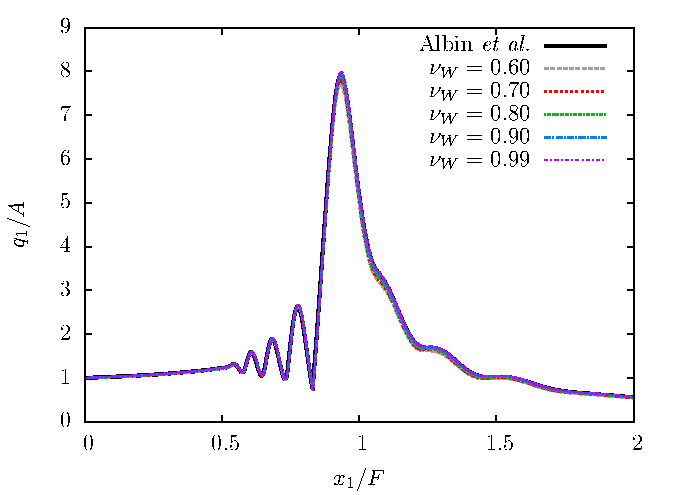
\includegraphics{7.pdf}
  }
} 
\caption{Focused wave, on axis pressure maximum for $a=30$, $\eta=82$, and different values of $\nu_W$. Reference values taken from Albin {\em et al.} \citep{albin} (color online).}
\label{fig:hifu-u1max-a30}
\end{figure}
%%%%%%%%%%%
\begin{figure}[htb] 
\centering 
\framebox{
  \resizebox{3.3in}{!}{
    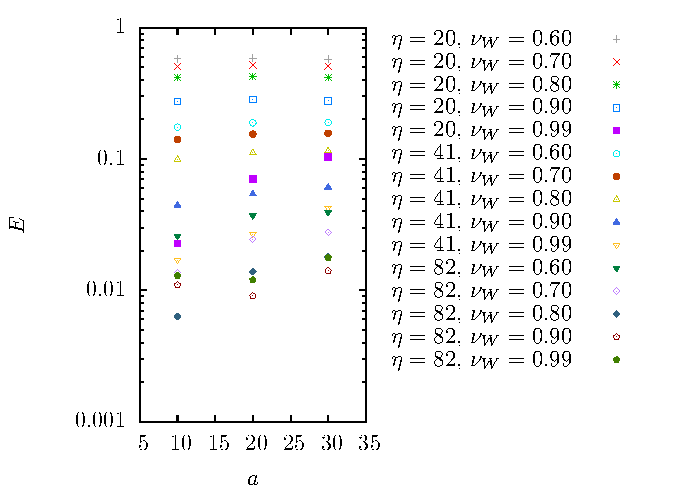
\includegraphics{8.pdf}
  }
} 
\caption{Focused wave, error for different values of $a$, $\nu_W$, and $\eta$ (color online).}
\label{fig:hifu-error}
\end{figure}

For this second test the results of Albin {\em et al.} \citep{albin} were used as reference, and simulation conditions were reproduced as closely as possible.

The boundary conditions for this simulation vary according to the region:
for the first stage, and when $x_1=0$ and $0\leq~x_2~\leq~a$, where $a$ is just a constant that is interpreted below, the boundary conditions are obtained by means of
\begin{subequations}
  \label{eq:hifuBC}
  \begin{align}
    q_1(0,x_2,t) &= 1+g \p{,} \\
    q_2(0,x_2,t) &= \frac{F g}{\sqrt{x_2^2 + F^2}} \p{,} \\
    q_3(0,x_2,t) &= \frac{-x_2 g}{ \sqrt{x_2^2 + F^2} } \p{,} \\ 
    g(x_2,t) &= 
    A  \sin\left(2\pi\tau \right)
    e^{ -\left( \frac{1}{4}\tau\right)^{-10}} \p{,} 
  \end{align}
\end{subequations}
where $ \tau = t + \frac{x_2^2}{2F}$, with parameters
\begin{align*}
  F = 50
  \p{,} \quad
  A = 4.217\times 10^{-4} 
  \p{,} \\
  \tilde{\delta} = 2.974 \times 10^{-4}
  \p{,}  \quad
  \beta = 4.8
  \p{.} 
\end{align*}
For the rest of the left border ($x_1=0$, $a < x_2$), and the top and right borders, a zero-order extrapolation has been used, which is a simplified version of absorbing boundaries \citep{leveque-book-fv}, p. 131.
The bottom border, which is treated in a reflective manner, makes use of the symmetry of the problem and reduces the calculations by half. 
In the second stage, the complete left border was taken to be a zero-order extrapolation and the other borders remained as they were.

These boundary conditions, particularly equations \eqref{eq:hifuBC}, correspond to parabolic approximation of a cylindrical symmetric wave packet entering the domain through a window of width $2a$, the center of this cylinder is the point $x_1=F$, $x_2=0$, but as can be seen in figures \ref{fig:hifu-u1max-a10}, \ref{fig:hifu-u1max-a20}, and \ref{fig:hifu-u1max-a30} (discussed below),  the focal point, corresponding to the global maximum, is slightly shifted toward $x_1=0$. 
In this case $L$, in equation \eqref{eq:renorm}, was taken to be equal to the wavelength, so that in dimensionless variables the wavelength is 1, and $\eta$ is the number of cells per wavelength.

Simulations were performed for the combinations of the following values: $a=10,20,30$, $\eta=20,41,82$, and $\nu_W=0.6,0.7,0.8,0.9,0.99$.  
As pointed in out in the previous section, the $\nu_W$ value does not exactly match the real CFL value, which led us to measure standard deviation as well, and it was in all cases lower than $10^{-4}$. 
All the simulations were performed up until a time value $t=100$, that is, until the wave packet had traveled a distance 100 times larger than the wavelength.
An upper view of a typical simulation is shown in figure \ref{fig:hifu-upper}.

The values reported by Albin {\em et al.} we have used to make comparisons are the pressure maximum over the propagation axis, with, in this case $x_2 = 0$. 
Since our equations \eqref{eq:OurSystem} are not written in terms of pressure, as are the results we are using for comparison, the first order approximation $p = c_0^2 \rho$ was used, which means that our $q^1$ variable corresponds to their ratio $\frac{p}{p_0}$. 
In order to avoid a transitory state, the maximum pressure was measured using the central peak in the wave packet. 

The comparison between schemes is illustrated, for pressure maximum over the propagation axis, using our finest mesh ($\eta=82$) in figures \ref{fig:hifu-u1max-a10}, \ref{fig:hifu-u1max-a20}, and \ref{fig:hifu-u1max-a30}. 
The lobe structure in the aforementioned figures, {\em e.g.} from $x_1=0.5$ to $x_1=0.8$ in the case $a=30$ (figure \ref{fig:hifu-u1max-a30}), is a consequence of the interaction of the wave packet we introduce, and which can be identified in figure \ref{fig:hifu-upper} as the high contrast line pattern, with an edge wave formed at $x_1=0$, $x_2=\pm a$, because of diffraction, and which is represented in figure \ref{fig:hifu-upper} by means of lighter line patterns.
The error analysis shown in figure \ref{fig:hifu-error} was calculated using expression \eqref{eq:error} and integrating over the $x_1$-axis.
In this case the error tends to zero when $\eta \rightarrow \infty$, which corresponds to a refinement of the mesh, and it is under $4\%$ for all cases with the finest mesh, $\eta=82$. 
Moreover, $E$ has a non-monotonic behavior as a function of $\nu_W$, but does not exhibit large variations within the $\nu_W$ tested range, which is qualitatively better for values tending to $\nu_W=1$. 
Thus, for the case $\eta=82$ we conclude that a very good agreement is obtained.



\subsection{Performance}
\label{sec:performance}

\begin{table}

  \begin{tabular}{ll|l|l|c}
    \cline{3-5}
    & & $\eta$ & $\nu_W$ & 
    \multicolumn{1}{c|}{execution time} \\ \hline
    \multicolumn{1}{|l|}{
    \multirow{2}{*}{\parbox{75pt}{Taylor shock, \\
Section~\ref{sec:agains-analyt-solut}}}} 
    & shortest & 20 & 0.99 & 
    \multicolumn{1}{c|}{12s} \\ \cline{2-5}
    \multicolumn{1}{ |c|  }{} 
    & longest  & 82 & 0.6  & 
    \multicolumn{1}{c|}{6min}  \\ \hline
    \multicolumn{1}{|l|}{
    \multirow{2}{*}{\parbox{75pt}{HIFU, \\
Section~\ref{sec:agains-anoth-numer}}}}            
    & shortest & 20 & 0.99 & 
    \multicolumn{1}{c|}{55s} \\ \cline{2-5}
    \multicolumn{1}{|c|}{} 
    & longest  & 82 & 0.6  & 
    \multicolumn{1}{c|}{47min} \\ \hline
    \end{tabular}
    \caption{Shortest and longest execution times.}
    \label{tab:times}
\end{table}

To make a performance comparison, a simulation was done with both a standard serial fortran CLAWPACK \citep{clawpack} 4.6.1 code and the C++/CUDA code described above.
A $256\times256$ mesh was used, with the first stage code only, and parameters
\begin{align*}
  \beta &= 4 
  \p{,} \qquad
  \tilde{\delta} = 10^{-7} 
  \p{,} \qquad
  L=\lambda
  \p{,} \qquad
  \text{$\eta$}=20
  \p{.}
\end{align*}
In the case where no data was written to disk and no plots were generated, the time execution factor, speedup, was of the order of $60$. 
In practice, one needs to store and plot some partial results all the time, however.
Taking this into account, this factor can increase to values over 100 because GPU execution does not need to go through the disk in order to display a plot. 
A different CUDA finite volume implementation, CUDACLAW \citep{cudaclaw}, has reported an execution time improvement of $30$ for CUDA execution over fortran execution. The discrepancy with regards to our case could be due to the fact that different CPU processors were used, i7 in their case, and i3 in our case.
The shortest and longest execution times for the simulations presented in the previous sections are listed in Table~\ref{tab:times}.

With relation to the reference results \citep{albin} we have used in Section~\ref{sec:agains-anoth-numer}, authors report they have used a mesh with approximately $21$ points per wavelength, and CFL values of $1/40$ for the firs stage, and $1/10$ for the second stage. 
In a rough comparison with our case corresponding to $\eta=82$, $\nu_W=0.99$, with a value of the error $E$ under $2\%$, it is noticeable that the total amount of spatiotemporal points for two spatial dimensions is only $1.5$ and $6$ times larger in our case, for first and second stage, respectively.
Albin {\em et al.} report for this case an execution time of $14$ min, on a 128 core cluster -- this is approximately a half of the execution time in our case, $31$ min, where the code is run on a single machine.

\section{Discussion and conclusions}
\label{sec:disc-concl}

A system of balance laws has been presented which constitutes a full wave model for nonlinear propagation at least as general as the Westervelt equation. 
This system of balance laws is well suited for use with a finite volume method, which we have  implemented using the Roe linearization. 
In the present work we have produced a two dimensional scheme, but the equations presented in Section~\ref{sec:equations} and Appendix~\ref{sec:appendix} can be used directly for a three dimensional generalization. 
In future stages of this work, the technical aspects of this implementation will be addressed. 
Moreover, the set of equations \eqref{eq:OurSystem} could also be implemented using other time or frequency domain numeric methods.

Although we have considered a homogeneous medium, the method could potentially be used in cases where the nonlinearity, $\beta$, and diffusivity, $\delta$, parameters have a smooth dependence on spatial coordinates, as long as this dependence does not invalidate the hypotheses used to obtain equations \eqref{eq:OurSystem}. 
Likewise, under the restrictions of the model listed in Section~\ref{sec:equations}, the presented method can be applied to a variety systems where nonlinear propagation is present: 
HIFU, 
ultrasound imaging, 
parametric acoustic arrays, 
oblique shock interactions,
propagation in waveguides \citep{rendon2010nonlinear}, 
and underwater acoustics. 

Recent applications using ultrasound imaging \citep{pinton2009heterogeneous, okita2011development} show that visualization is an important tool for understanding complex phenomena, and implementation on GPU systems allows for quick visualization of the acoustic field, linear or nonlinear. 
In this way, GPU implementation could constitute an important tool for understanding a variety of acoustic phenomena.

The validation tests performed for the numeric method show a very good agreement with references, especially with the finest mesh ($\eta=82$). 
In the case of a plane wave analytic solution, the measured error was under $1\%$, and in the case of full wave propagation it was under $\%2$. 
The performance of the scheme presented in this work compares favorably with the recent method we have used as reference \citep{albin} -- execution times are comparable even taking into account that our scheme is executed in a single machine equipped with a GPU, as opposed to a full-fledged cluster.
Some recent publications on frequency domain methods claim that one advantage of this approach is the execution time optimization, due to the larger point separation that can be achieved for its meshes \citep{albin, huijssen2010iterative}. 
However, even in this case, having different approaches to model the same system is handy because it permits the validation of numeric results, as is the case here.

Even if execution times for the present work are already not large, as can be seen in Table \ref{tab:times},  finer meshes could not be used because of memory limitations of the GPU. 
This limitation could be overcome with parallel execution between GPUs. 
Then, to take advantage of parallelized code, GPU execution should be integrated in cluster systems with tools like OpenMP and MPI. 

In results not reported here, we have seen single precision implementations sometimes offer results as good as those obtained with double precision calculation.
The advantage we have observed in those cases is that single precision calculation improves the execution time for our code and hardware by a factor of approximately $1.5$ -- the difference could be larger given a different hardware configuration.

A simplified version of this code 
%%% \MDbegin{journalX twoColumnB phone preprint twoColumnA tablet}
is publicly available under a free and open-source software (FOSS) license in the temporary address \url{https://github.com/rvelseg/FiVoNAGI}.
%%% \MDend{journalX twoColumnB phone preprint twoColumnA tablet}
%%% \MDbegin{arXiv}
% will be publicly available under a free and open-source software (FOSS) license in the temporary address \url{https://github.com/rvelseg/FiVoNAGI}, when this publication is ready.
%%% \MDend{arXiv}
The name of the repository stands for Finite Volume Nonlinear Acoustics GPU Implementation. This version of the code is capable of reproducing the results reported in this paper. As a precedent, there are other nonlinear acoustic codes published as FOSS \citep{frijlink2008abersim,anderson20002d}.

\section{Acknowledgments}
\label{sec:acknowledges}

The authors are grateful to Dr. Felipe Ordu\~{n}a for his useful comments, 
to the CLAWPACK \citep{clawpack} project for sharing their base code, 
to Dr. Randy LeVeque for the useful information provided, 
and to Dr. Oscar P. Bruno, Dr. Nathan Albin, and coworkers for kindly providing comparison data.
This work was financially supported by PAPIIT 110411, PAEP UNAM 2011-2013, and Conacyt M\'{e}xico.

\appendix

\section{Balance laws derivation}
\label{sec:appendix}

In this section we describe the details of the obtention of the system of equations \eqref{eq:OurSystem}.
This procedure is analogous to that described by Hamilton and Morfey to obtain the Westervelt equation \citep{hamilton1998model}.

Acoustics is a theory which describes small mechanical deviations from a given state in a particular medium;
in the words of Beyer, it is an {\em infinitesimal theory} \citep{beyer}, p. 1.
Here, we use, as is standard practice, the Mach number $\epsilon$, defined as the ratio of the magnitude $u$ of fluid velocity $\mathbf{u}$ to the speed of sound of small signals $c_0$, 
\begin{align*}
  \epsilon = \frac{u}{c_0}
  \p{,}
\end{align*} 
as a small parameter upon which we base our perturbative approach.

Crucially, we assume the following ratios to be not only small, but $O(\epsilon)$ as well
\begin{align*}
  \epsilon 
  \approx \frac{\rho'}{\rho_0}
  \approx \frac{p'}{p_0}
  \approx \frac{T'}{T_0}
  \p{,}
\end{align*}
As usual, the subscript $0$ refers to the equilibrium state, which here we assume constant, and the prime superscript refers to a small perturbation of said equilibrium: $\rho= \rho_0 + \rho'$ is mass density, $p = p_0 + p'$ is the pressure, and $T = T_0 + T'$ is the temperature. We take the equilibrium state for $\mathbf{u}$ to be zero.

After examination of the energy conservation equation, it becomes evident that one scaling parameter is not enough and further assumptions on the scaling of the problem are necessary.
In this case we assume $s'$, the perturbed entropy per unit mass, to be small as well.

Our starting point is the following set of conservation laws:
\begin{align} 
  \label{eq:ap:mass}
  \frac{\partial \rho}{\partial t} + \nabla \cdot
  \left(\rho \mathbf{u}\right)& = 0 
  \p{,} \\ 
  \label{eq:ap:mom}
  \Dp{\rho \mathbf{u}}{t} +
  \nabla\cdot\rho\mathbf{u}\otimes\mathbf{u}
  + \nabla p 
  & = 
  \left(\frac{4}{3}\mu + \mu_B\right)\nabla^2\mathbf{u}
  \p{,} \\ 
  \label{eq:ap:ener}
  \rho_0 T_0 \Dp{s'}{t} &= \kappa \nabla^2 T'
  \p{.}
\end{align}
Equation \eqref{eq:ap:mass} is the continuity equation as presented in Section 2 of Hamilton and Morfey \citep{hamilton1998model}; 
the force balance equation \eqref{eq:ap:mom}, where $\mu$ is dynamic viscosity, $\mu_B$ is bulk viscosity, and $\otimes$ denotes outer product, has been written for a Newtonian fluid with irrotational flow ($\nabla\times\mathbf{u}=0$), and is equivalent to eq. (32), again in Hamilton and Morfey \citep{hamilton1998model}; 
and finally, the energy conservation equation \eqref{eq:ap:ener}, or in this case entropy equation, is written in such a way that only the linear acoustic mode term remains, (33) in the same reference \citep{hamilton1998model}.

Now, because of the number of variables compared with the number of equations, we consider two equations of state, $p=p(\rho,s)$ and $T=T(\rho,s)$.
Without giving a specific form to the dependency, following Hamilton and Morfey \citep{hamilton1998model}, we choose to write their Taylor series to second order for the former and to first order for the latter
\begin{align*}
  p' &= 
  c_0^2 \rho' + c_0^2 \frac{1}{\rho_0} \frac{B}{2A}(\rho')^2 +
  \left(\Dp{p}{s}\right)_{\rho,0} s' \\
  & \qquad
  + \Dpp{^2 p}{\rho\partial s}_0 s' \rho'
  + \frac{1}{2} \Dpp{^2 p}{s^2}_{\rho,0} (s')^2
  \p{,} \\  
  T' &= \left(\Dp{T}{\rho}\right)_{s,0} \rho'
  + \Dpp{T}{s}_{\rho,0} s'
  \p{,}
\end{align*}
where $c_0$, $A$, and $B$ have the usual definitions \citep{beyer},
\begin{align}
  c_0^2 &= \Dpp{p}{\rho}_{s,0} 
  \p{,} \\
  A &= \rho_0 \Dpp{p}{\rho}_{s,0} 
  \p{,} \quad
  B = \rho_0^2 \Dpp{^2p}{\rho^2}_{s,0} 
  \p{.} 
\end{align}
As pointed out by Hamilton and Morfey, the entropy perturbations $s'$ are order $\epsilon^2$ far from the boundary layers, which allows us to neglect the cross term ($\epsilon s'$) in eq. \eqref{eq:EOS:p}, and the linear term $s'$ for eq. \eqref{eq:EOS:T}:
\begin{align}
  \label{eq:EOS:p}
  p' &= 
  c_0^2 \rho' + c_0^2 \frac{1}{\rho_0} \frac{B}{2A}(\rho')^2 +
  \left(\Dp{p}{s}\right)_{\rho,0} s' 
  \p{,} \\  
  \label{eq:EOS:T}
  T' &= \left(\Dp{T}{\rho}\right)_{s,0} \rho'
  \p{.}
\end{align}

Now consider the following linear relations: the first order $p$ equation of state evaluated at equilibrium,
\begin{align}
  \label{eq:EOSzero}
  p_0 &= c_0^2 \rho_0 
  \p{,}
\end{align}
the linearized version of the continuity equation,
\begin{align}
  \label{eq:LMcons}
  \nabla\cdot\mathbf{u} &= \frac{-1}{\rho_0}\Dp{\rho'}{t}
  \p{,}
\end{align}
and the linear inviscid wave equation for temperature,
\begin{align}
  \label{eq:waveT}
  \nabla^2 T' &= c_0^{-2} \Dp{^2T'}{t^2} \p{.}
\end{align}
Then, substituting expressions \eqref{eq:ap:ener}, \eqref{eq:EOSzero}, \eqref{eq:LMcons}, \eqref{eq:waveT}, the thermodynamic property \citep{foot1}
\begin{align*}
  c_v - c_p = \frac{TV\alpha^2}{N\kappa_T}  
  \p{,}
\end{align*}
and the following Maxwell relations, see Callen \citep{callen2006thermodynamics}, Chap. 7,
\begin{align*} 
\Dpp{p}{T}_V &= \Dpp{S}{V}_T \p{,} 
\Dpp{p}{S}_V = -\Dpp{T}{V}_S \p{,} \\ 
\Dpp{V}{T}_p &= -\Dpp{S}{p}_T 
\end{align*}
into \eqref{eq:EOS:p}, we get, after some algebra,
\begin{align}
  \label{eq:finalp}
  p = c_0^2 \rho + c_0^2 \frac{1}{\rho_0} \frac{B}{2A}(\rho')^2 +
  \frac{\kappa}{\rho_0}
  \left(
    \frac{1}{c_v} - \frac{1}{c_p}
  \right)
  \rho_0 \nabla\cdot\mathbf{u}
  \p{.}
\end{align}

Direct substitution of \eqref{eq:finalp} into \eqref{eq:ap:mom}, taking into account that $\rho\mathbf{u}\otimes\mathbf{u}$ can be written $\rho_0\mathbf{u}\otimes\mathbf{u}$ at $O(\epsilon^2)$, leads us to the final form of the equations \eqref{eq:OurSystem}:
\begin{align*} 
  \frac{\partial \rho}{\partial t} + \nabla \cdot
  \left(\rho \mathbf{u}\right)& = 0 
  \p{,} \\ 
  \Dp{\rho \mathbf{u}}{t} +
  \nabla\cdot\left(
    \rho_0 \mathbf{u}\otimes\mathbf{u} + \mathbf{I}\tilde{p}
  \right)
  &= 
  \rho_0 \delta \nabla^2 \mathbf{u}
  \p{,} \\
  \tilde{p} = 
  c_0^2 \rho + \frac{c_0^2}{\rho_0} (\beta-1)(\rho-\rho_0)^2 
  \p{,}
\end{align*}
where $\mathbf{I}$ is a $3\times 3$ identity matrix,
\begin{align}
\label{eq:def-delta}
  \delta = \frac{1}{\rho_0}
  \left(
    \frac{4}{3}
    \mu+\mu_B
  \right)
  +
  \frac{\kappa}{\rho_0}
  \left(
    \frac{1}{c_v}
    -\frac{1}{c_p}
  \right)
\end{align}
is Lighthill's  acoustic diffusivity \citep{lighthill}, and
\begin{align*}
  \beta = 1 + \frac{B}{2A}
\end{align*}
is the nonlinear coefficient \citep{beyer1998parameter}.

%%% \MDbegin{arXiv twoColumnA}
% \section*{References}
%%% \MDend{arXiv twoColumnA}

\bibliographystyle{unsrtnat}
\bibliography{references}
%C-c .

%%% The following commands will only work if the bib-at-work
%%% package is used, see the begining of document.
%%
%% \rule{2px}{7px}~{\tt{}Keys not in reference list}:
%% \biblostkeys~\rule{2px}{7px}
%%
%% \rule{2px}{7px}~{\tt{}Keys not cited in text}:
%% \refnotcalled~\rule{2px}{7px}

\end{document}

%%%%%% emacs
%%%%%%%%%%%%
%%% Local Variables:
%%% ispell-local-dictionary: "en_US"
%%% TeX-PDF-mode: t
%%% eval: (auto-fill-mode -1)
%%% mode: whitespace-newline
%%% mode: visual-line
%%% fill-column: 64
%%% End:

%%%%%%%%%%%%%%%% ispell
%%%%%%%%%%%%%%%%%%%%%%%
% LocalWords: CLAWPACK asymptotical  parallelized FOSS FiVoNAGI
% LocalWords: Westervelt KZK lithotripsy Wendroff eigenvectors
% LocalWords: irrotational GPU Albin CFL Morfey RHS
% LocalWords: HIFU CUDA undimensionalized Lighthill Hopf KdV fv
% LocalWords: Kuznetsov diagonalizable Fubini  renormalization
% LocalWords: Blackstock Navier fortran adimensional 
% LocalWords: suberboom PAPIIT Conacyt PAEP linearizations eq
% LocalWords: Jacobian GPL  Beyer nonlinearity inviscid
% LocalWords: propagations Laplacian obtention linearized 
% LocalWords: compressibility isothermal Lighthill's https et
% LocalWords: diagonalizability  eigenvector al GPUs 
% LocalWords: LeVeque's LeVeque overcomed extracorporeal MPI
% LocalWords: pseudospectral Christov lossless
% LocalWords: linearization  thermoviscous OpenMP perturbative
% LocalWords: diffusivity OpenCL  Aanonsen UNAM
% LocalWords: analytical  Callen waveguides comparables
% LocalWords: spatiotemporal dissipative
